%%%%%%%% ICML 2023 EXAMPLE LATEX SUBMISSION FILE %%%%%%%%%%%%%%%%%

\documentclass{article}

% Recommended, but optional, packages for figures and better typesetting:
\usepackage{microtype}
\usepackage{graphicx}
\usepackage{tikz}
\usepackage{subfigure}
\usepackage{booktabs} % for professional tables

% hyperref makes hyperlinks in the resulting PDF.
% If your build breaks (sometimes temporarily if a hyperlink spans a page)
% please comment out the following usepackage line and replace
% \usepackage{icml2023} with \usepackage[nohyperref]{icml2023} above.
\usepackage{hyperref}


% Attempt to make hyperref and algorithmic work together better:
\newcommand{\theHalgorithm}{\arabic{algorithm}}

% Use the following line for the initial blind version submitted for review:
\usepackage{icml2023}

% If accepted, instead use the following line for the camera-ready submission:
% \usepackage[accepted]{icml2023}

% For theorems and such
\usepackage{amsmath}
\usepackage{amssymb}
\usepackage{mathtools}
\usepackage{amsthm}

% if you use cleveref..
\usepackage[capitalize,noabbrev]{cleveref}

%%%%% NEW MATH DEFINITIONS %%%%%

\usepackage{amsmath,amsfonts,bm}

% Mark sections of captions for referring to divisions of figures
\newcommand{\figleft}{{\em (Left)}}
\newcommand{\figcenter}{{\em (Center)}}
\newcommand{\figright}{{\em (Right)}}
\newcommand{\figtop}{{\em (Top)}}
\newcommand{\figbottom}{{\em (Bottom)}}
\newcommand{\captiona}{{\em (a)}}
\newcommand{\captionb}{{\em (b)}}
\newcommand{\captionc}{{\em (c)}}
\newcommand{\captiond}{{\em (d)}}

% Highlight a newly defined term
\newcommand{\newterm}[1]{{\bf #1}}


% Figure reference, lower-case.
\def\figref#1{Figure~\ref{#1}}
% Figure reference, capital. For start of sentence
\def\Figref#1{Figure~\ref{#1}}
\def\twofigref#1#2{figures \ref{#1} and \ref{#2}}
\def\quadfigref#1#2#3#4{figures \ref{#1}, \ref{#2}, \ref{#3} and \ref{#4}}
% Section reference, lower-case.
\def\secref#1{section~\ref{#1}}
% Section reference, capital.
\def\Secref#1{Section~\ref{#1}}
% Reference to two sections.
\def\twosecrefs#1#2{sections \ref{#1} and \ref{#2}}
% Reference to three sections.
\def\secrefs#1#2#3{sections \ref{#1}, \ref{#2} and \ref{#3}}
% Reference to an equation, lower-case.
% \def\eqref#1{\eqref{#1}}
% Reference to an equation, upper case
% \def\Eqref#1{Equation~\ref{#1}}
% A raw reference to an equation---avoid using if possible
\def\plaineqref#1{\ref{#1}}
% Reference to a chapter, lower-case.
\def\chapref#1{chapter~\ref{#1}}
% Reference to an equation, upper case.
\def\Chapref#1{Chapter~\ref{#1}}
% Reference to a range of chapters
\def\rangechapref#1#2{chapters\ref{#1}--\ref{#2}}
% Reference to an algorithm, lower-case.
\def\algref#1{algorithm~\ref{#1}}
% Reference to an algorithm, upper case.
\def\Algref#1{Algorithm~\ref{#1}}
\def\twoalgref#1#2{algorithms \ref{#1} and \ref{#2}}
\def\Twoalgref#1#2{Algorithms \ref{#1} and \ref{#2}}
% Reference to a part, lower case
\def\partref#1{part~\ref{#1}}
% Reference to a part, upper case
\def\Partref#1{Part~\ref{#1}}
\def\twopartref#1#2{parts \ref{#1} and \ref{#2}}

\def\ceil#1{\lceil #1 \rceil}
\def\floor#1{\lfloor #1 \rfloor}
\def\1{\bm{1}}
\newcommand{\train}{\mathcal{D}}
\newcommand{\valid}{\mathcal{D_{\mathrm{valid}}}}
\newcommand{\test}{\mathcal{D_{\mathrm{test}}}}

\def\eps{{\epsilon}}


% Random variables
\def\reta{{\textnormal{$\eta$}}}
\def\ra{{\textnormal{a}}}
\def\rb{{\textnormal{b}}}
\def\rc{{\textnormal{c}}}
\def\rd{{\textnormal{d}}}
\def\re{{\textnormal{e}}}
\def\rf{{\textnormal{f}}}
\def\rg{{\textnormal{g}}}
\def\rh{{\textnormal{h}}}
\def\ri{{\textnormal{i}}}
\def\rj{{\textnormal{j}}}
\def\rk{{\textnormal{k}}}
\def\rl{{\textnormal{l}}}
% rm is already a command, just don't name any random variables m
\def\rn{{\textnormal{n}}}
\def\ro{{\textnormal{o}}}
\def\rp{{\textnormal{p}}}
\def\rq{{\textnormal{q}}}
\def\rr{{\textnormal{r}}}
\def\rs{{\textnormal{s}}}
\def\rt{{\textnormal{t}}}
\def\ru{{\textnormal{u}}}
\def\rv{{\textnormal{v}}}
\def\rw{{\textnormal{w}}}
\def\rx{{\textnormal{x}}}
\def\ry{{\textnormal{y}}}
\def\rz{{\textnormal{z}}}

% Random vectors
\def\rvepsilon{{\mathbf{\epsilon}}}
\def\rvtheta{{\mathbf{\theta}}}
\def\rva{{\mathbf{a}}}
\def\rvb{{\mathbf{b}}}
\def\rvc{{\mathbf{c}}}
\def\rvd{{\mathbf{d}}}
\def\rve{{\mathbf{e}}}
\def\rvf{{\mathbf{f}}}
\def\rvg{{\mathbf{g}}}
\def\rvh{{\mathbf{h}}}
\def\rvu{{\mathbf{i}}}
\def\rvj{{\mathbf{j}}}
\def\rvk{{\mathbf{k}}}
\def\rvl{{\mathbf{l}}}
\def\rvm{{\mathbf{m}}}
\def\rvn{{\mathbf{n}}}
\def\rvo{{\mathbf{o}}}
\def\rvp{{\mathbf{p}}}
\def\rvq{{\mathbf{q}}}
\def\rvr{{\mathbf{r}}}
\def\rvs{{\mathbf{s}}}
\def\rvt{{\mathbf{t}}}
\def\rvu{{\mathbf{u}}}
\def\rvv{{\mathbf{v}}}
\def\rvw{{\mathbf{w}}}
\def\rvx{{\mathbf{x}}}
\def\rvy{{\mathbf{y}}}
\def\rvz{{\mathbf{z}}}
\def\rvzeta{{\mathbf{\zeta}}}

% Elements of random vectors
\def\erva{{\textnormal{a}}}
\def\ervb{{\textnormal{b}}}
\def\ervc{{\textnormal{c}}}
\def\ervd{{\textnormal{d}}}
\def\erve{{\textnormal{e}}}
\def\ervf{{\textnormal{f}}}
\def\ervg{{\textnormal{g}}}
\def\ervh{{\textnormal{h}}}
\def\ervi{{\textnormal{i}}}
\def\ervj{{\textnormal{j}}}
\def\ervk{{\textnormal{k}}}
\def\ervl{{\textnormal{l}}}
\def\ervm{{\textnormal{m}}}
\def\ervn{{\textnormal{n}}}
\def\ervo{{\textnormal{o}}}
\def\ervp{{\textnormal{p}}}
\def\ervq{{\textnormal{q}}}
\def\ervr{{\textnormal{r}}}
\def\ervs{{\textnormal{s}}}
\def\ervt{{\textnormal{t}}}
\def\ervu{{\textnormal{u}}}
\def\ervv{{\textnormal{v}}}
\def\ervw{{\textnormal{w}}}
\def\ervx{{\textnormal{x}}}
\def\ervy{{\textnormal{y}}}
\def\ervz{{\textnormal{z}}}

% Random matrices
\def\rmA{{\mathbf{A}}}
\def\rmB{{\mathbf{B}}}
\def\rmC{{\mathbf{C}}}
\def\rmD{{\mathbf{D}}}
\def\rmE{{\mathbf{E}}}
\def\rmF{{\mathbf{F}}}
\def\rmG{{\mathbf{G}}}
\def\rmH{{\mathbf{H}}}
\def\rmI{{\mathbf{I}}}
\def\rmJ{{\mathbf{J}}}
\def\rmK{{\mathbf{K}}}
\def\rmL{{\mathbf{L}}}
\def\rmM{{\mathbf{M}}}
\def\rmN{{\mathbf{N}}}
\def\rmO{{\mathbf{O}}}
\def\rmP{{\mathbf{P}}}
\def\rmQ{{\mathbf{Q}}}
\def\rmR{{\mathbf{R}}}
\def\rmS{{\mathbf{S}}}
\def\rmT{{\mathbf{T}}}
\def\rmU{{\mathbf{U}}}
\def\rmV{{\mathbf{V}}}
\def\rmW{{\mathbf{W}}}
\def\rmX{{\mathbf{X}}}
\def\rmY{{\mathbf{Y}}}
\def\rmZ{{\mathbf{Z}}}

% Elements of random matrices
\def\ermA{{\textnormal{A}}}
\def\ermB{{\textnormal{B}}}
\def\ermC{{\textnormal{C}}}
\def\ermD{{\textnormal{D}}}
\def\ermE{{\textnormal{E}}}
\def\ermF{{\textnormal{F}}}
\def\ermG{{\textnormal{G}}}
\def\ermH{{\textnormal{H}}}
\def\ermI{{\textnormal{I}}}
\def\ermJ{{\textnormal{J}}}
\def\ermK{{\textnormal{K}}}
\def\ermL{{\textnormal{L}}}
\def\ermM{{\textnormal{M}}}
\def\ermN{{\textnormal{N}}}
\def\ermO{{\textnormal{O}}}
\def\ermP{{\textnormal{P}}}
\def\ermQ{{\textnormal{Q}}}
\def\ermR{{\textnormal{R}}}
\def\ermS{{\textnormal{S}}}
\def\ermT{{\textnormal{T}}}
\def\ermU{{\textnormal{U}}}
\def\ermV{{\textnormal{V}}}
\def\ermW{{\textnormal{W}}}
\def\ermX{{\textnormal{X}}}
\def\ermY{{\textnormal{Y}}}
\def\ermZ{{\textnormal{Z}}}

% Vectors
\def\vzero{{\bm{0}}}
\def\vone{{\bm{1}}}
\def\vmu{{\bm{\mu}}}
\def\vtheta{{\bm{\theta}}}
\def\va{{\bm{a}}}
\def\vb{{\bm{b}}}
\def\vc{{\bm{c}}}
\def\vd{{\bm{d}}}
\def\ve{{\bm{e}}}
\def\vf{{\bm{f}}}
\def\vg{{\bm{g}}}
\def\vh{{\bm{h}}}
\def\vi{{\bm{i}}}
\def\vj{{\bm{j}}}
\def\vk{{\bm{k}}}
\def\vl{{\bm{l}}}
\def\vm{{\bm{m}}}
\def\vn{{\bm{n}}}
\def\vo{{\bm{o}}}
\def\vp{{\bm{p}}}
\def\vq{{\bm{q}}}
\def\vr{{\bm{r}}}
\def\vs{{\bm{s}}}
\def\vt{{\bm{t}}}
\def\vu{{\bm{u}}}
\def\vv{{\bm{v}}}
\def\vw{{\bm{w}}}
\def\vx{{\bm{x}}}
\def\vy{{\bm{y}}}
\def\vz{{\bm{z}}}

% Elements of vectors
\def\evalpha{{\alpha}}
\def\evbeta{{\beta}}
\def\evepsilon{{\epsilon}}
\def\evlambda{{\lambda}}
\def\evomega{{\omega}}
\def\evmu{{\mu}}
\def\evpsi{{\psi}}
\def\evsigma{{\sigma}}
\def\evtheta{{\theta}}
\def\eva{{a}}
\def\evb{{b}}
\def\evc{{c}}
\def\evd{{d}}
\def\eve{{e}}
\def\evf{{f}}
\def\evg{{g}}
\def\evh{{h}}
\def\evi{{i}}
\def\evj{{j}}
\def\evk{{k}}
\def\evl{{l}}
\def\evm{{m}}
\def\evn{{n}}
\def\evo{{o}}
\def\evp{{p}}
\def\evq{{q}}
\def\evr{{r}}
\def\evs{{s}}
\def\evt{{t}}
\def\evu{{u}}
\def\evv{{v}}
\def\evw{{w}}
\def\evx{{x}}
\def\evy{{y}}
\def\evz{{z}}

% Matrix
\def\mA{{\bm{A}}}
\def\mB{{\bm{B}}}
\def\mC{{\bm{C}}}
\def\mD{{\bm{D}}}
\def\mE{{\bm{E}}}
\def\mF{{\bm{F}}}
\def\mG{{\bm{G}}}
\def\mH{{\bm{H}}}
\def\mI{{\bm{I}}}
\def\mJ{{\bm{J}}}
\def\mK{{\bm{K}}}
\def\mL{{\bm{L}}}
\def\mM{{\bm{M}}}
\def\mN{{\bm{N}}}
\def\mO{{\bm{O}}}
\def\mP{{\bm{P}}}
\def\mQ{{\bm{Q}}}
\def\mR{{\bm{R}}}
\def\mS{{\bm{S}}}
\def\mT{{\bm{T}}}
\def\mU{{\bm{U}}}
\def\mV{{\bm{V}}}
\def\mW{{\bm{W}}}
\def\mX{{\bm{X}}}
\def\mY{{\bm{Y}}}
\def\mZ{{\bm{Z}}}
\def\mBeta{{\bm{\beta}}}
\def\mPhi{{\bm{\Phi}}}
\def\mLambda{{\bm{\Lambda}}}
\def\mSigma{{\bm{\Sigma}}}

% Tensor
\DeclareMathAlphabet{\mathsfit}{\encodingdefault}{\sfdefault}{m}{sl}
\SetMathAlphabet{\mathsfit}{bold}{\encodingdefault}{\sfdefault}{bx}{n}
\newcommand{\tens}[1]{\bm{\mathsfit{#1}}}
\def\tA{{\tens{A}}}
\def\tB{{\tens{B}}}
\def\tC{{\tens{C}}}
\def\tD{{\tens{D}}}
\def\tE{{\tens{E}}}
\def\tF{{\tens{F}}}
\def\tG{{\tens{G}}}
\def\tH{{\tens{H}}}
\def\tI{{\tens{I}}}
\def\tJ{{\tens{J}}}
\def\tK{{\tens{K}}}
\def\tL{{\tens{L}}}
\def\tM{{\tens{M}}}
\def\tN{{\tens{N}}}
\def\tO{{\tens{O}}}
\def\tP{{\tens{P}}}
\def\tQ{{\tens{Q}}}
\def\tR{{\tens{R}}}
\def\tS{{\tens{S}}}
\def\tT{{\tens{T}}}
\def\tU{{\tens{U}}}
\def\tV{{\tens{V}}}
\def\tW{{\tens{W}}}
\def\tX{{\tens{X}}}
\def\tY{{\tens{Y}}}
\def\tZ{{\tens{Z}}}


% Graph
\def\gA{{\mathcal{A}}}
\def\gB{{\mathcal{B}}}
\def\gC{{\mathcal{C}}}
\def\gD{{\mathcal{D}}}
\def\gE{{\mathcal{E}}}
\def\gF{{\mathcal{F}}}
\def\gG{{\mathcal{G}}}
\def\gH{{\mathcal{H}}}
\def\gI{{\mathcal{I}}}
\def\gJ{{\mathcal{J}}}
\def\gK{{\mathcal{K}}}
\def\gL{{\mathcal{L}}}
\def\gM{{\mathcal{M}}}
\def\gN{{\mathcal{N}}}
\def\gO{{\mathcal{O}}}
\def\gP{{\mathcal{P}}}
\def\gQ{{\mathcal{Q}}}
\def\gR{{\mathcal{R}}}
\def\gS{{\mathcal{S}}}
\def\gT{{\mathcal{T}}}
\def\gU{{\mathcal{U}}}
\def\gV{{\mathcal{V}}}
\def\gW{{\mathcal{W}}}
\def\gX{{\mathcal{X}}}
\def\gY{{\mathcal{Y}}}
\def\gZ{{\mathcal{Z}}}

% Sets
\def\sA{{\mathbb{A}}}
\def\sB{{\mathbb{B}}}
\def\sC{{\mathbb{C}}}
\def\sD{{\mathbb{D}}}
% Don't use a set called E, because this would be the same as our symbol
% for expectation.
\def\sF{{\mathbb{F}}}
\def\sG{{\mathbb{G}}}
\def\sH{{\mathbb{H}}}
\def\sI{{\mathbb{I}}}
\def\sJ{{\mathbb{J}}}
\def\sK{{\mathbb{K}}}
\def\sL{{\mathbb{L}}}
\def\sM{{\mathbb{M}}}
\def\sN{{\mathbb{N}}}
\def\sO{{\mathbb{O}}}
\def\sP{{\mathbb{P}}}
\def\sQ{{\mathbb{Q}}}
\def\sR{{\mathbb{R}}}
\def\sS{{\mathbb{S}}}
\def\sT{{\mathbb{T}}}
\def\sU{{\mathbb{U}}}
\def\sV{{\mathbb{V}}}
\def\sW{{\mathbb{W}}}
\def\sX{{\mathbb{X}}}
\def\sY{{\mathbb{Y}}}
\def\sZ{{\mathbb{Z}}}

% Entries of a matrix
\def\emLambda{{\Lambda}}
\def\emA{{A}}
\def\emB{{B}}
\def\emC{{C}}
\def\emD{{D}}
\def\emE{{E}}
\def\emF{{F}}
\def\emG{{G}}
\def\emH{{H}}
\def\emI{{I}}
\def\emJ{{J}}
\def\emK{{K}}
\def\emL{{L}}
\def\emM{{M}}
\def\emN{{N}}
\def\emO{{O}}
\def\emP{{P}}
\def\emQ{{Q}}
\def\emR{{R}}
\def\emS{{S}}
\def\emT{{T}}
\def\emU{{U}}
\def\emV{{V}}
\def\emW{{W}}
\def\emX{{X}}
\def\emY{{Y}}
\def\emZ{{Z}}
\def\emSigma{{\Sigma}}

% entries of a tensor
% Same font as tensor, without \bm wrapper
\newcommand{\etens}[1]{\mathsfit{#1}}
\def\etLambda{{\etens{\Lambda}}}
\def\etA{{\etens{A}}}
\def\etB{{\etens{B}}}
\def\etC{{\etens{C}}}
\def\etD{{\etens{D}}}
\def\etE{{\etens{E}}}
\def\etF{{\etens{F}}}
\def\etG{{\etens{G}}}
\def\etH{{\etens{H}}}
\def\etI{{\etens{I}}}
\def\etJ{{\etens{J}}}
\def\etK{{\etens{K}}}
\def\etL{{\etens{L}}}
\def\etM{{\etens{M}}}
\def\etN{{\etens{N}}}
\def\etO{{\etens{O}}}
\def\etP{{\etens{P}}}
\def\etQ{{\etens{Q}}}
\def\etR{{\etens{R}}}
\def\etS{{\etens{S}}}
\def\etT{{\etens{T}}}
\def\etU{{\etens{U}}}
\def\etV{{\etens{V}}}
\def\etW{{\etens{W}}}
\def\etX{{\etens{X}}}
\def\etY{{\etens{Y}}}
\def\etZ{{\etens{Z}}}

% The true underlying data generating distribution
\newcommand{\pdata}{p_{\rm{data}}}
% The empirical distribution defined by the training set
\newcommand{\ptrain}{\hat{p}_{\rm{data}}}
\newcommand{\Ptrain}{\hat{P}_{\rm{data}}}
% The model distribution
\newcommand{\pmodel}{p_{\rm{model}}}
\newcommand{\Pmodel}{P_{\rm{model}}}
\newcommand{\ptildemodel}{\tilde{p}_{\rm{model}}}
% Stochastic autoencoder distributions
\newcommand{\pencode}{p_{\rm{encoder}}}
\newcommand{\pdecode}{p_{\rm{decoder}}}
\newcommand{\precons}{p_{\rm{reconstruct}}}

\newcommand{\laplace}{\mathrm{Laplace}} % Laplace distribution

\newcommand{\E}{\mathbb{E}}
\newcommand{\Ls}{\mathcal{L}}
\newcommand{\R}{\mathbb{R}}
\newcommand{\emp}{\tilde{p}}
\newcommand{\lr}{\alpha}
\newcommand{\reg}{\lambda}
\newcommand{\rect}{\mathrm{rectifier}}
\newcommand{\softmax}{\mathrm{softmax}}
\newcommand{\sigmoid}{\sigma}
\newcommand{\softplus}{\zeta}
\newcommand{\KL}{D_{\mathrm{KL}}}
\newcommand{\Var}{\mathrm{Var}}
\newcommand{\standarderror}{\mathrm{SE}}
\newcommand{\Cov}{\mathrm{Cov}}
% Wolfram Mathworld says $L^2$ is for function spaces and $\ell^2$ is for vectors
% But then they seem to use $L^2$ for vectors throughout the site, and so does
% wikipedia.
\newcommand{\normlzero}{L^0}
\newcommand{\normlone}{L^1}
\newcommand{\normltwo}{L^2}
\newcommand{\normlp}{L^p}
\newcommand{\normmax}{L^\infty}

\newcommand{\parents}{Pa} % See usage in notation.tex. Chosen to match Daphne's book.

\DeclareMathOperator*{\argmax}{arg\,max}
\DeclareMathOperator*{\argmin}{arg\,min}

\DeclareMathOperator{\sign}{sign}
\DeclareMathOperator{\Tr}{Tr}
\let\ab\allowbreak

% custom commands
\newcommand{\todo}[1]{{\color{red}\textbf{TODO:}``#1''}}
% \newcommand{\R}{\mathbb{R}}
\newcommand{\N}{\mathbb{N}}
\renewcommand{\P}{\mathbb{P}}
\newcommand{\C}{\mathcal{C}}
\renewcommand{\L}{\mathrm{L}}
\newcommand{\dx}{\mathrm{d}}
\newcommand{\X}{\mathcal{X}}
\newcommand{\Z}{\mathcal{Z}}
\newcommand{\T}{\mathcal{T}}
\newcommand{\id}{\mathrm{Id}}
\newcommand{\norm}[1]{\left\Vert#1\right\Vert}
\newcommand{\scal}[2]{\left\langle#1,#2\right\rangle}
\renewcommand{\vec}[1]{\mathbf{#1}}
\newcommand{\diameter}{\mathrm{diam}}
\newcommand{\prox}{\mathrm{prox}}
\newcommand{\proj}{\mathrm{proj}}
\newcommand{\tmin}{t_\mathrm{min}}
\newcommand{\tmax}{t_\mathrm{max}}
% \newcommand{\hatt}{\widehat{t}}
\def\hatt{{\widehat{t}}}
\newcommand{\tminh}{\hatt_\mathrm{min}}
\newcommand{\tmaxh}{\hatt_\mathrm{max}}

% \newcommand{\E}{\mathbb{E}}
\newcommand{\dist}[1]{\mathcal{P}_{#1}}
\newcommand{\pdf}[1]{p_{#1}}
\newcommand{\g}{\vert}
\newcommand{\normal}{\mathcal{N}}

\newcommand{\VP}{\mathrm{VP}}
\newcommand{\VE}{\mathrm{VE}}

%%%%%%%%%%%%%%%%%%%%%%%%%%%%%%%%
% THEOREMS
%%%%%%%%%%%%%%%%%%%%%%%%%%%%%%%%
\theoremstyle{plain}
\newtheorem{theorem}{Theorem}[section]
\newtheorem{proposition}[theorem]{Proposition}
\newtheorem{lemma}[theorem]{Lemma}
\newtheorem{corollary}[theorem]{Corollary}
\theoremstyle{definition}
\newtheorem{definition}[theorem]{Definition}
\newtheorem{assumption}[theorem]{Assumption}
\theoremstyle{remark}
\newtheorem{remark}[theorem]{Remark}

% Todonotes is useful during development; simply uncomment the next line
%    and comment out the line below the next line to turn off comments
%\usepackage[disable,textsize=tiny]{todonotes}
% \usepackage[textsize=tiny]{todonotes}


% The \icmltitle you define below is probably too long as a header.
% Therefore, a short form for the running title is supplied here:
\icmltitlerunning{Learned Diffusion Models Follow Graduated Non-Convexity Principle}

\begin{document}

\twocolumn[
\icmltitle{Learned Diffusion Models Follow Graduated Non-Convexity Principle}

% It is OKAY to include author information, even for blind
% submissions: the style file will automatically remove it for you
% unless you've provided the [accepted] option to the icml2023
% package.

% List of affiliations: The first argument should be a (short)
% identifier you will use later to specify author affiliations
% Academic affiliations should list Department, University, City, Region, Country
% Industry affiliations should list Company, City, Region, Country

% You can specify symbols, otherwise they are numbered in order.
% Ideally, you should not use this facility. Affiliations will be numbered
% in order of appearance and this is the preferred way.
\icmlsetsymbol{equal}{*}

\begin{icmlauthorlist}
\icmlauthor{Firstname1 Lastname1}{equal,yyy}
\icmlauthor{Firstname2 Lastname2}{equal,yyy,comp}
\icmlauthor{Firstname3 Lastname3}{comp}
\icmlauthor{Firstname4 Lastname4}{sch}
\icmlauthor{Firstname5 Lastname5}{yyy}
\icmlauthor{Firstname6 Lastname6}{sch,yyy,comp}
\icmlauthor{Firstname7 Lastname7}{comp}
%\icmlauthor{}{sch}
\icmlauthor{Firstname8 Lastname8}{sch}
\icmlauthor{Firstname8 Lastname8}{yyy,comp}
%\icmlauthor{}{sch}
%\icmlauthor{}{sch}
\end{icmlauthorlist}

\icmlaffiliation{yyy}{Department of XXX, University of YYY, Location, Country}
\icmlaffiliation{comp}{Company Name, Location, Country}
\icmlaffiliation{sch}{School of ZZZ, Institute of WWW, Location, Country}

\icmlcorrespondingauthor{Firstname1 Lastname1}{first1.last1@xxx.edu}
\icmlcorrespondingauthor{Firstname2 Lastname2}{first2.last2@www.uk}

% You may provide any keywords that you
% find helpful for describing your paper; these are used to populate
% the "keywords" metadata in the PDF but will not be shown in the document
\icmlkeywords{Machine Learning, ICML}

\vskip 0.3in
]

% this must go after the closing bracket ] following \twocolumn[ ...

% This command actually creates the footnote in the first column
% listing the affiliations and the copyright notice.
% The command takes one argument, which is text to display at the start of the footnote.
% The \icmlEqualContribution command is standard text for equal contribution.
% Remove it (just {}) if you do not need this facility.

%\printAffiliationsAndNotice{}  % leave blank if no need to mention equal contribution
\printAffiliationsAndNotice{\icmlEqualContribution} % otherwise use the standard text.

\begin{abstract}
This document provides a basic paper template and submission guidelines.
Abstracts must be a single paragraph, ideally between 4--6 sentences long.
Gross violations will trigger corrections at the camera-ready phase.
\end{abstract}

First implementation of diffusion based models~\cite{SoJa15}; newly discovered and leading to remarkable image generation results~\cite{HoJa20,SoEr20,RoBl22}

\cite{NiDh21} improved training strategy 


Variational diffusion models~\cite{KiSa21} showed the equivalence of diffusion models (noise preserving, noise exploding, \ldots) in continuous time.


Continuous Diffusion for Categorical Data (CDCD)~\cite{DiSa22} space and time continuous by score interpolation in time and time warping to adapt the capacity of model over time (Jonas Adler).


Learning maximal monotone operators~\cite{PeRe21, TeRe21}


TODO:
\begin{itemize}
    \item in eq (3) remove dependency of $\theta$ or $R_L$
\end{itemize}

% -----------------------------------------------------------------------------------------------------
\section{Introduction}

Main points:
\begin{itemize}
    \item DM actually learn GNC scheme
    \item We show effectiveness of GNC on a simple example, i.e., smaller number of steps are required to obtain the global minimum
    \item 
    \item relation to variational networks
    \item it is not clear if the score networks implement a gradient, thus we parameterize the energy directly
\end{itemize}

% -----------------------------------------------------------------------------------------------------
\section{Background}

\begin{itemize}
    \item diffusion based model (how do they incorporate the smoothing parameter)
    \item TNRDs and VNs
    \item plug and play priors
\end{itemize}

\subsection{Variational Networks}
Introduction and definition of unrolling approach in particular for variational networks.

\subsection{Score Matching}

What do the others do with the $t$ parameter.

variational analysis of denoising diffusion models~\cite{HuLi21}

% -----------------------------------------------------------------------------------------------------
\section{A Graduated Non-convexity View of Denoising Diffusion-based Models} \label{sec:gnc}
Let $(\X,\mathfrak{F},\P)$ be a complete probability space on a compact set~$\X\subset\R^d$ with sigma algebra~$\mathfrak{F}$ and probability measure~$\P$.
We further assume an absolutely continuous probability measure with corresponding probability density function~$\pdf{\rvx}\in \C_0(\X,[0,\infty))$.
Later, we will also consider a discrete probability measure defined by the empirical distribution of a dataset~$\{\vx_i\}_{i=1}^n\subset\X$ with cardinality~$n\in\N$.
In addition, we consider variances~$t\in\T$, with the compact interval~$\T=[\tmin,\tmax]$ where $0<\tmin<\tmax<\infty$.

In this setting, we show that noise-conditional score matching (NCSM)~\citep{SoEr19} as well as denoising diffusion probabilistic models (DDPM)~\citep{HoJa20} actually learn a graduated non-convexity (GNC) scheme~\citep{BlZi87}.
In detail, both NCSM and DDPM train a neural network to learn a conditional score, i.e., the gradient of the log density of the data degraded by additive Gaussian noise with variance~$t$.
The conditioning is either directly on the variance (NCSM) or a diffusion time (DDPM), which encodes the variance.
The key observation is that although the data becomes noisier with increasing~$t$, the corresponding smooth probability density~$\pdf{\rvx\vert\rt}$ gets smoother and its associated energy~$F(\vx,t)=-\log\pdf{\rvx\vert\rt}(\vx,t)$ gets more \emph{convex}, see the left plot in Figure~\ref{fig:gmmOptimization}.
Next, we prove that in the considered setting there indeed exists a lower bound on the variance~$\widetilde{t}$ such that the energy of the conditional density is convex for~$t\geq\widetilde{t}$.

Before diving into the proof, we first introduce multivariate Gaussians and Gaussian mixture models for completeness.
Let $G(\bm{\mu},\Sigma)$ denote a multivariate Gaussian probability density with mean~$\bm{\mu}\in\R^d$ and symmetric positive definite covariance matrix~$\Sigma\in\R^{d\times d}$, which reads as
\[
G(\bm{\mu},\Sigma)(\vx)=\vert 2\pi\Sigma\vert^{-\frac{1}{2}}\exp\left(-\norm{\vx-\bm{\mu}}_{\Sigma^{-1}}^2\right).
\]
\begin{definition}[GMM]
Let $n\in\N$.
A Gaussian mixture model (GMM) consisting of $n$ weighted normal distributions is defined as
\[
p = \sum_{i=1}^n w_i G(\vx_i,\Sigma_i)
\]
with mean vectors $\{\vx_i\}_{i=1}^n\subset\R^d$ and positive semidefinite covariance matrices~$\{\Sigma_i\}_{i=1}^n\subset\R^{d\times d}$.
All mixture weights are positive and sum up to~$1$, i.e., $(w_1\ \cdots\ w_n)^\top\in\Delta^n$.
\end{definition}
Recall that for $n\to\infty$ a GMM can uniformly approximate any function in~$\C_0$~\citep{NgNg20}.
Note that an approximation w.r.t.~$\L^p$ also holds for any~$p_X\in\L^p$ for~$p\in[1.\infty)$.
Consequently, our setting and most practically encountered probability density functions can be well approximated by GMMs.
Thus, we focus in the following proof on probability density functions induced by a GMM.

\begin{theorem}\label{thm:Fconvex}
Let~$\X\subset\R^d$ be a bounded set such that diameter~$\diameter(\X)<\infty$ and consider a GMM of the form
\[
p(\vx) = \sum_{i=1}^n w_i G(\vx_i,\Sigma_i)(\vx),
\]
where $(w_1\ \cdots \ w_n)^\top\in\Delta^n$. Assume~$\{\vx_i\}_{i=1}^n\subset\X$.
Then there exists a smoothing parameter~$\widetilde{t}\in(0,\infty)$ such that the smoothed energy
\[
F(\vx,t)\coloneqq -\log \big( (p \ast G(\vec{0}, t\id))(\vx)\big)
\]
is \emph{convex} w.r.t.~$\vx$ for all~$t\geq\widetilde{t}$.
\end{theorem}
\begin{corollary}\label{cor:empirical}
Theorem~\ref{thm:Fconvex} also holds if an empirical discrete probability measure of a dataset~$\{\vx_i\}_{i=1}^n\subset\X$, i.e.
\[
p = \frac{1}{n}\sum_{i=1}^n\delta_{\vx_i},
\]
is considered.
Here, $\delta_{\vx}$ denotes the Dirac delta measure located at~$\vx$.
\end{corollary}
The proofs of the theorem and corollary can be found in~\cref{apdx:proofs}.
Note that in this paper we only consider the variance exploding setting, however, similar results can be obtained for variance preserving schemes~\citep{SoSo20}. 

The underlying idea of the graduated non-convexity algorithm is to speed up the estimation of the global minimum of a non-convex energy.
First, this energy is approximated by a one-parameter family of energies that become more convex for increasing~$t$.
Second, an initial smoothing parameter is selected such that the energy is convex.
Third, the initial problem is efficiently solved due to increased smoothness and convexity.
Then, the parameter is reduced such that the energy becomes gradually more non-convex.
The resulting energy is minimized using the previous solution as initialization and the process is repeated until convergence of the energy corresponding to the smallest parameter.

Comparing NCSM and DDPM to GNC, we observe the following similarities:
First, the score networks also approximate a one-parameter family of the gradient of associated energies.
Second, the schedule of the smoothing parameter is a priori fixed, for instance, by the variance schedule of an annealed Langevin algorithm~\citep{SoEr19} or the diffusion time~\citep{HoJa20}.
Finally, as we proved above, there exists a smoothing parameter such that the associated energy becomes convex in most practical cases.

To combine the best of both approaches, we propose the annealed GNC scheme described in~\Algref{alg:graduatedNC}.
In particular, we first fix a decreasing sequence of smoothing parameters~$\{t_i\}_{i=0}^I$ such that the enegy~$F(\vx,t_0)$ is convex.
Due to smoothness and convexity, we know that the conditional minimal MSE estimator~$\vx^1$ computed by Tweedie's identity~\citep{Ro56,Ef11} is close to the mode of~$F(\vx,t_0)$.
Then this estimator is gradually refined by reducing the smoothing~$t_{i-1}<t_i$ and updating the MMSE estimator conditioned on the previous result.

\begin{algorithm}[t]
\caption{Annealed graduated non-convexity scheme for minimizing a smoothed family of energies~$F(\vx,t)$}\label{alg:graduatedNC}
\textbf{Step 0:} Take~$I\in\N$, choose sequence $\{t_i\}_{i=0}^I\subset[\tmin,\tmax]$ s.t.~$t_{i}>t_{i+1}$ and~$F(\vx,t_0)$ convex, $\vx_0\in\X$, $\eta>0$ \\
\textbf{Step i:} $(0\leq i< I)$ 
Approximately minimize current energy~$F(\cdot,t_i)$ using single step
\[
\vx_{i+1}=\vx_i-t_i\eta \nabla_\vx F(\vx_i,t_i)
\] 
\end{algorithm}

\begin{figure}[th]
\centering
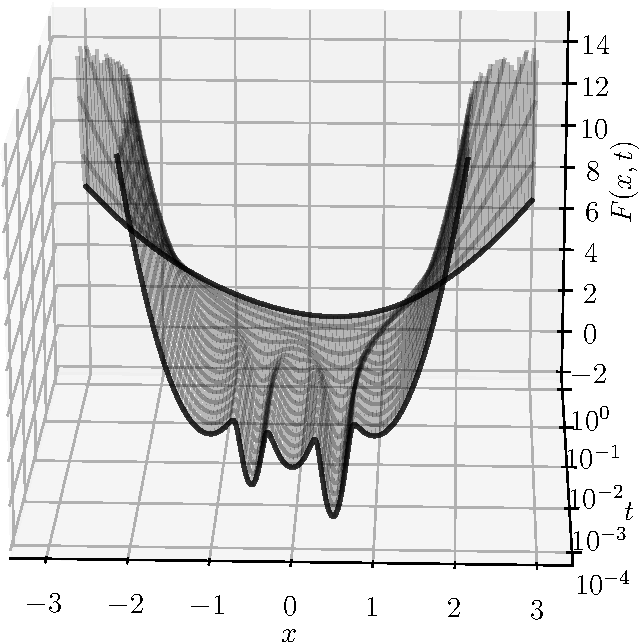
\includegraphics[width=.7\linewidth]{./figures/ex_gmm/ex_gmm_func}\\[1em]
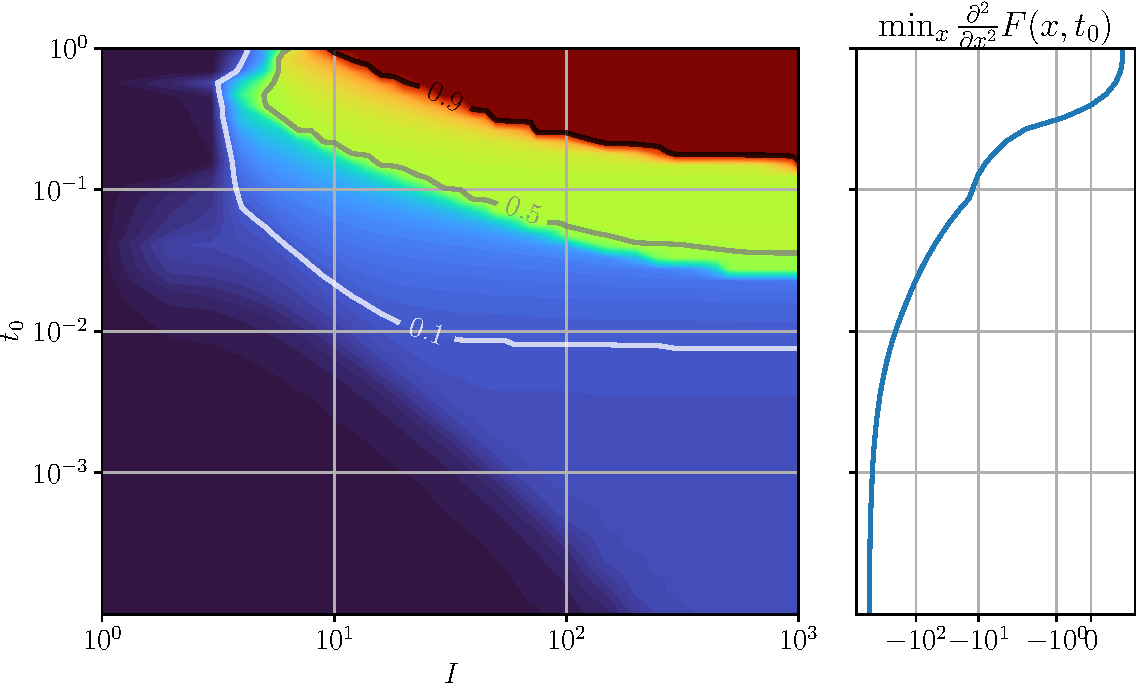
\includegraphics[width=.85\linewidth]{./figures/ex_gmm/ex_gmm_rate}
\label{fig:gmmOptimization}
\caption{Top: Illustration of the 1D example energy~\eqref{eq:gmmEx} using gray lines for different~$t\in[10^{-4},1]$.
Center: Visualization of the rate of trajectories attaining the global minimum at~$x=\frac{1}{2}$ using~$N=1\ 000$ equally spaced initial points as a function of the initial smoothing time~$t_0$ for a different number of steps~$I$.
The larger the initial smoothing parameter~$t_0$, the fewer steps are required to obtain the perfect rate.
Bottom: If the smallest second derivative of~$F$ w.r.t.~$x$ is positive anywhere for~$t_0$, it is convex.
}
\end{figure}
To illustrate the effectiveness of the annealed GNC approach, we consider a simple 1D example.
In particular, we use the smoothed GMM corresponding to the energy
\begin{align} \label{eq:gmmEx}
F(x,t)=-\log\left(\sum_{i=1}^5 w_i G\left(\mu_i,\sigma_i^2+t\right)(x)\right)
\end{align}
consisting of five components over the domain $x\in[-3,3]$ and $t\in[10^{-4},1]$.
The detailed parameters are~$\bm{w}=\tfrac{1}{100}(5\ 15\ 15\ 60\ 5)$, $\bm{\mu}=(-1\ -\tfrac12\ 0\ \tfrac12\ 1)$, and $\bm{\sigma}^2=\tfrac{1}{100}(10\ 1\ 5\ 1\ 10)$.
Note that the addition of $t$ at the variances in~\eqref{eq:gmmEx} originates from the convolution of the data density with a Gaussian as considered in Theorem~\ref{thm:Fconvex}.
This energy is illustrated by the black lines at the top in~\figref{fig:gmmOptimization} for various~$t$.
As can be seen, increasing the smoothing parameter~$t$ results in smoother and more convex energies.

The plot in the center of \figref{fig:gmmOptimization} visualizes the rate of trajectories converging to the global minimum at~$x=\tfrac12$ as a function of the initial smoothing~$t_0$ and the number of performed steps~$I$.
For each~$t_0$ all trajectories start from~$N=1\ 000$ equally spaced initial positions~$x^0$ on $[-3,3]$ and are defined by performing $I$~annealed GNC steps using a logarithmic smoothing schedule.
By comparing the different contour lines we observe that for larger initial smoothing fewer steps are required such that all trajectories converge to the global minimum.
This highlights the effectiveness of the GNC approach.
Finally, the bottom plot in \figref{fig:gmmOptimization} depicts the smallest~$\frac{\partial^2}{\partial x^2}F(x,t_0)$ and thereby highlights convexity of~$F$ as a function of~$t_0$.

% -----------------------------------------------------------------------------------------------------
\section{Learning Priors on the Space of Images}
In this section, we transfer the insights gained from relations of graduated non-convexity and diffusion-based models to learn priors on the space of images.
In this space, an image is simply a point in a high-dimensional space with a dimension equal to the number of image pixels.

\subsection{Prior Models for the Space of Image Patches}
Let $\vx\in\X\subset\R^d$ be an image patch of size~$d=m\times n\times c$, where $m$ represents its height, $n$ its width, and $c$ is the number of feature channels.
Without loss of generality, we consider the input domain~$\X=[a,b]^d$ for $a<b$ and $a,b\in\R$.
A popular choice is $a=0$ and $b=1$.
Note that this domain can be obtained by a simple preprocessing step for many imaging applications.
The domain of the smoothing parameter is fixed to~$\T=[\tmin,\tmax]$, where~$0<\tmin<\tmax<\infty$.
We commonly set~$\tmin=10^{-4}$ and $\tmax=1$.

\subsubsection{Extending the Fields of Experts}
\citet{RoBl09} introduced a simple and versatile prior operating on image patches called fields of experts~(FoE).
This prior has been successfully applied to various inverse problems in imaging sciences and its essential building blocks are (local) convolutions that extract lower-level features as well as non-linear potential functions.
In particular, we consider the FoE model
\[
R_\mathrm{FoE}(\vx) = \scal{\vec{1}}{\left(\Phi \circ K\right)(\vx)},
\]
where the linear operator~$K\colon\R^d\to\R^{d_1}$ extracts~$N_1$ features using 2D convolution kernels~$k_i$ with~$d_1=m\times n\times N_1$.
The operator~$\Phi\colon\R^{d_1}\to\R^{d_1}$ applies to every feature channel~$k_i(\vx)$ a corresponding pixel-wise parametric non-linear function~$\phi_i\colon\R\to\R$, and the scalar product denotes the sum over all pixels and channels.
The underlying idea is that every convolution kernel~$k_i$ specializes on a certain pattern and the associated non-linearity~$\phi_i$ describes the corresponding energy, i.e., the negative logarithm of the density.
The non-linear functions~$\phi_i$ are typically learnable and implemented by simple parametric functions~\citep{RoBl09,ChRa14} or weighted radial basis functions~\citep{ChPo16,KoKl17}.
Originally, \citet{RoBl09} learned the parameters (convolution kernels, and weights of the potential functions) using contrastive divergence~\citep{Hi02}.

Motivated by the results of the previous section, we next extend the FoE prior to the space of images by introducing the smoothing parameter~$t$.
In detail, the extended FoE reads as
\begin{align}\label{eq:r1}
R_1(\vx,t) = \scal{\vec{1}}{\left(\Phi_1(\cdot, t) \circ K_1\right)(\vx)},
\end{align}
where the non-linear function depends on~$t$, i.e., $\Phi_1\in\C^3(\R^{d_1}\times\T,\R^{d_1})$.
Consequently, also the pixel-wise non-linear functions of every feature channel~$\phi_{1j}\in\C^3(\R\times\T,\R)$, $j=1,\ldots,N_1$ depend on~$t$. 
Further, all~$\phi_{1j}$ are constructed using weighted 2D quartic spline basis functions, which are equally distributed over the input domain to ensure sufficient smoothness for gradient-based learning.
We refer to \cref{apdx:implementationDetails} for further details regarding the spline-based non-linear functions.

\subsubsection{Increasing Depth}
Since the prior~\eqref{eq:r1} essentially consists of a single layer, its expressiveness is limited to simple image features.
To overcome this limitation, we propose to stack multiple convolutions and parametric non-linear layers.
Then, an FoE-type prior facilitating $L$-layers reads as
\[
R_L(\vx,t) = \scal{\vec{1}}{\left(\Phi_L(\cdot,t)\circ K_L\circ\cdots\circ\Phi_1(\cdot, t) \circ K_1\right)(\vx)}.
\]
Each convolution~$K_i\colon\R^{d_{i-1}}\to\R^{d_i}$, $i=1,\ldots,L$ performs a linear combination of all input features, thereby enabling the mixing of features as typically performed in convolutional neural networks (CNNs).
In contrast to typical CNNs, we use parametric activation functions that adapt to the corresponding feature channels.
At every layer~$i\in\{1,\ldots,L\}$ and for any feature channel~$j\in\{1,\ldots,N_i\}$, we employ a 2D parametric point-wise function~$\phi_{ij}\in\C^3(\R\times\T,\R)$ to non-linearly process the features.
Further details about the parametrization of the activation functions can be found in \cref{apdx:implementationDetails}.
This idea follows recent suggestions to facilitate spline-based parametric activation functions in deep CNNs~\citep{OcMe18,AzGu20}.


\subsection{Learning Parametric Models on the Space of Images}
Here, we elaborate on how to fit the parameters of the previously defined regularizers~$R_L\colon\X,\T,\Theta\to\R$ to the negative score of the \emph{joint} density~$\pdf{\rvy,\rt}:\X\times\T\to\R_+$ of the data.
For our previously defined degradation model, the joint density function reads as
\begin{align*}
\pdf{\rvy,\rt}(\vy,t) &= \left(\pdf{\rvx}\ast G(\vec{0},t\id)\right)(\vy) \pdf{\rt}(t)\\
&\propto \E_{\vx\sim\dist{X}}\left[\exp\left(-\frac{\norm{\vy-\vx}_2^2}{2 t}\right)\right] \pdf{\rt}(t),
\end{align*}
where $\pdf{\rt}$ is the prior of the smoothing parameter.
Then, the objective function of (explicit) score matching is given by
\begin{align} \label{eq:jsm}
&J_\mathrm{SM}(\theta) = \\
&\hspace{1ex}\E_{\vy,t\sim\dist{Y,T}}\left[\tfrac12\norm{\nabla R_L(\vy,t;\theta) -\left(- \nabla\log p_{\rvy,T}(\vy,\rt)\right)}_M^2\right], \notag
\end{align}
where $\nabla$ denotes the full gradient of a function and an additional index denotes the gradient w.r.t. only this variable and 
$M\in\R^{d+1\times d+1}$ is a positive definite block-diagonal matrix, i.e.,
\[
M = \begin{pmatrix}
t\id & \vec{0} \\
\vec{0}^T & m_t
\end{pmatrix}.
\]
By applying the metric, we obtain
\begin{align}\label{eq:jsmParts}
&J_\mathrm{SM}(\theta)=\\
&\hspace{1ex}\E_{\vy,t\sim\dist{Y,T}}\Big[\tfrac{t}{2}\norm{\nabla_\vy R_L(\vy,t;\theta) -\left(- \nabla_\vy\log p_{Y,T}(\vy,t)\right)}_2^2 \notag\\
&\hspace{6ex}+\tfrac12\left(\tfrac{\partial}{\partial t}R_L(\vy,t;\theta) -\left(-\tfrac{\partial}{\partial t}\log p_{Y,T}(\vy,t)\right)\right)^2m_t\Big].\notag
\end{align}
Note that~$J_\mathrm{SM}$ decouples into a score matching objective on noisy images~$\vy$ and the smoothing parameter~$t$; the metric (in particular~$m_T>0$) enables balancing of both terms.
The scaling of the first term by~$t$ is a common variance reduction technique in denoising score matching~\citep{SoEr19,HuLi21}.

To avoid the computation of the expectation over the true data in the gradient of the joint distribution, we apply denoising score matching to the noisy image term.
In addition, we replace the score matching objective w.r.t.~$t$ by its implicit pendant and get
\begin{align*}
&J_\mathrm{SM}(\theta)=\\
&\hspace{1ex}\E_{\vx,\vy,t\sim\dist{X,Y,T}}\left[\tfrac{t}{2}\norm{\nabla_\vy R_L(\vy,t;\theta) -\tfrac{1}{t}(\vy-\vx)}_2^2 \right.\\
&\hspace{5ex}+ \left. \tfrac{m_t}{2}\left(\left(\tfrac{\partial}{\partial t}R_L(\vy,t;\theta)\right)^2 -2\tfrac{\partial^2}{\partial t^2}R_L(\vy,t;\theta)\right)\right] + C,
\end{align*}
where $C$ is an additive constant.
The proof can be obtained by combining the equivalence proofs of~\citet{Hy05} and~\citet{Vi11}.
To further simply the objective, we perform the change of variables~$\vy=\vx+\sqrt{t}\vn$, where~$\vn\sim\mathcal{N}(\vec{0},\id)$.
Then, we get the equivalent loss function
\begin{align} \label{eq:loss}
&J(\theta)=\\
&\hspace{1ex}\E_{\vx,\vn,t\sim\dist{X,N,T}}\tfrac{1}{2}\left[\norm{\sqrt{t}\nabla_\vy R_L(\vy,t;\theta) -\vn}_2^2\right. \notag\\ 
&\hspace{9ex}\left.+m_t\left(\left(\tfrac{\partial}{\partial t}R_L(\vy,t;\theta)\right)^2 -2\tfrac{\partial^2}{\partial t^2}R_L(\vy,t;\theta)\right)\right]. \notag
\end{align}
In contrast to pure denoising score matching-based loss functions~\citep{SoEr19,HoJa20}, the loss~\eqref{eq:loss} introduces a regularization along the smoothing direction~$t$.
In particular, the loss favors energies~$R_L$ that slowly change in this direction and are preferably convex.
Note that these properties are desirable for any gradient-based optimization scheme operating on the joint energy~$F$.

\subsubsection{Logarithmic Reparametrization}
The score-matching-based training ensures that the non-linear functions better approximate the score of the true data of the features as~$t\to\tmin$.
Thus, it is reasonable to distribute the learnable weights of~$\phi_i$ toward this regime to account for the increasing complexity.
Therefore, we facilitate the logarithmic reparametrization~$\widehat{t}=\log(t)$, $\tminh=\log(\tmin)$, and $\tmaxh=\log(\tmax)$, as suggested by~\citet{KaMi22}.
Then, the domain~$\widehat{\T}$ is on the negative halfspace and the loss~\eqref{eq:loss} changes to
\begin{align} \label{eq:losslog}
&\widehat{J}(\theta)=\\
&\hspace{1ex}\E_{\vx,\vn,\widehat{t}\sim\dist{X,N,\widehat{T}}}\tfrac12\Bigg[\norm{e^{\widehat{t}/2}\nabla_\vy R_L(\vy,\widehat{t};\theta) -\vn}_2^2 \notag\\
&\hspace{11ex}+ \left(\left(\tfrac{\partial}{\partial\widehat{t}}R_L(\vy,\widehat{t};\theta)\right)^2 -2\tfrac{\partial^2}{\partial \widehat{t}^2}R_L(\vy,\widehat{t};\theta)\right)\Bigg]. \notag
\end{align}
We highlight that the gradient and the Hessian are measured on the logarithmic domain to avoid intensive regularization toward~$\tmin$.


\section{Solving Inverse Problems using Priors on the Space of Images}
In various imaging applications, the task is to determine an underlying image~$\rvx$ given observations~$\rvz$.
The observations are related to the target through the forward problem
\[
\rvz = A \rvx + \rvzeta
\]
where the random variable~$\rvzeta$ represents additive noise and the operator~$A$ describes the measurement process.
The simplest example is image denoising, where the operator~$A=\id$ and the distribution of~$\rvzeta$ describe the noise type.
In the case of image inpainting, the operator~$A$ applies a binary mask to every image element, which is 1 if the associated pixel is observed and 0 otherwise, and~$\rvzeta\equiv\vec{0}$.

Frequently, the maximum a posteriori estimator is computed to approximate the target, which amounts to
\[
\max_{\vx\in\X}\left\{\pdf{\rvx\vert\rvz}(\vx\vert\vz)\propto \pdf{\rvz\vert\rvx}(\vz\vert\vx)\pdf{\rvx}(\vx)\right\}
\]
due to Bayes.
In the negative log domain, we get
\[
\min_{\vx\in\X}\left\{ -\log\pdf{\rvx}(\vx) -\log\pdf{\rvz\vert\rvx}(\vz\vert\vx) = R(\vx) + D(\vz,\vx)\right\},
\]
which is also known as the variational approach.
Here, the negative log-prior is equivalent to the regularizer~$R\colon\X\to\R$ and the negative log-likelihood equals the data fidelity term~$D\colon\Z\times\X\to\R$.
The data fidelity models the forward problem and ensures consistency to the observations, whereas, the regularizer incorporates prior (statistical) knowledge of the solution.
Throughout this section, we assume that the data fidelity term has a simple proximal mapping, which is the case for many inverse problems in imaging.
To utilize the statistical knowledge of our learned prior~$R_L$, we next describe suitable ways to handle the additional smoothing parameter~$\widehat{t}$.

\subsection{Joint Optimization} \label{sec:jointOptimization}
As presented in \secref{sec:gnc}, decreasing the smoothing parameter~$\widehat{t}$ results in peakier and more non-convex energies.
Thus, there are pronounced local minima at~$\tminh$ and $\frac{\partial}{\partial\widehat{t}}R_L$ is likely to point toward~$\tminh$.
Consequently, it is reasonable to minimize the joint energy also w.r.t. the smoothing parameter~$\widehat{t}$.
Thus, we seek to solve the optimization problem
\begin{align} \label{eq:jointEnergy}
\min_{\vx\in\X,\ \widehat{t}\in[\tminh,\tmaxh]} \left\{E(\vx,\widehat{t})\coloneqq R_L(\vx,\widehat{t}) + D(\vz,\vx)\right\}
\end{align}
using an alternating proximal gradient scheme~\citep{BoSa14} and Lipschitz backtracking of~\citet{BeTe09}.
The algorithm is summarized in~\algref{alg:jointMinimization}.

\begin{algorithm}[t]
\caption{Proximal alternating linearization method (PALM) with Lipschitz backtracking.}\label{alg:jointMinimization}
\textbf{Step 0:} Take $L_\vx^0,L_\hatt^0>0$, some~$\gamma_1,\gamma_2\in(0,1)$ and~$\vx^0\in\X$, $\hatt_0\in[\tminh,\tmaxh]$\\
\textbf{Step i:} $(i\geq 0)$ 
\begin{enumerate}
\item
Determine the smallest integer~$k_i$ such that 
\begin{align*}
R_L(\vx,\hatt_i) \leq &R_L(\vx_i,\hatt_i) + \scal{\nabla_\vx R_L(\vx_i,\hatt_i))}{\vx-\vx_i} \\
&+ \tfrac{1}{2\eta}\norm{\vx-\vx_i}_2^2
\end{align*}
with $\vx = \prox_{\eta D(\vz,\cdot)}(\vx_i-\eta\nabla_\vx R_L(\vx_i,\hatt_i))$ using $\eta=\tfrac{\gamma^{k_i}}{L_\vx^i}$.
\item
Set $\vx_{i+1}=\vx$ and $L_\vx^{i+1}=\max\left(\tfrac{\gamma_2}{\eta},1\right)$
\item
Determine the smallest integer~$l_i$ such that 
\begin{align*}
R_L(\vx_{i+1},\hatt) \leq &R_L(\vx_{i+1},\hatt_i) + \tfrac{\partial}{\partial\hatt} R_L(\vx_{i+1},\hatt_i)(\hatt-\hatt_i) \\
&+ \tfrac{1}{2\eta}(\hatt-\hatt_i)^2
\end{align*}
with $\hatt = \proj_{[\tminh,\tmaxh]}(\hatt_i-\eta\tfrac{\partial}{\partial\hatt}R_L(\vx_{i+1},\hatt_i))$ using $\eta=\tfrac{\gamma^{l_i}}{L_\hatt^i}$.
\item
Set $\hatt_{i+1}=\hatt$ and $L_\hatt^{i+1}=\max\left(\tfrac{\gamma_2}{\eta},1\right)$
\end{enumerate}
\end{algorithm}

\subsection{Predefined Smoothing Schedule} \label{sec:predefinedSchedule}
The second approach is motivated by recent DDPM models~\citep{SoEr19,HoJa20}.
The idea is to first define a decreasing schedule for smoothing parameters~$\{\widehat{t}_i\}_{i=1}^n$ such that~$\tmaxh>\widehat{t}_1$, $\widehat{t}_i>\widehat{t}_{i+1}$ for~$i=1,\ldots,n-1$ and $\widehat{t}_n=\tminh$.
Then, this sequence defines a family of optimization problems
\[
\vx_i =\argmin_{\vx\in\X} \left\{E(\widehat{t}_i)\coloneqq R_L(\vx,\widehat{t}_i)+D(\vz,\vx)\right\}
\]
that are sequentially minimized using the proximal gradient scheme~\citep{Be17}
\begin{align} \label{eq:fixedScheme}
\vx_{i+1} = \prox_{\eta_iD(\vz,\cdot)}(\vx_i-\eta_i\nabla_\vx R_L(\vx_i,\widehat{t}_i)),
\end{align}
where~$\eta_i$ is the step size at the~$i^\text{th}$ iteration.
Note that we perform only a single proximal-gradient step on every energy~$E(\widehat{t}_i)$ since the energies smoothly change along~$\widehat{t}$ for large enough~$n$.
For selecting the step sizes, we consider Tweedie's identity as in \secref{sec:gnc}.
In particular, Tweedie's formula states that a gradient step on the log density of noisy images (degraded by additive Gaussian noise) scaled by the variance results in the conditional mean squared estimator.
Using the training objective~\eqref{eq:losslog}, our priors learned to approximate the negative log-density of noisy image patches for any smoothing parameter~$\widetilde{t}$.
Thus, we obtain an approximation of the conditional mean estimator by setting the step size to an estimate of the variance~$\eta_i=\exp(\widehat{t}_i)$.
Note that the proximal mapping in~\eqref{eq:fixedScheme} ensures data consistency and thereby frequently reintroduces some noise into~$\vx_{i+1}$.

\subsection{Task-specifig Learning of Smoothing Schedule} \label{sec:learnedVN}
Since it is not clear how to choose the predefined smoothing scheduler~$\{\widehat{t}_i\}_{i=1}^n$, why not learn it from data for a specific task?
To do so, we propose to ``unroll'' the optimization scheme~\eqref{eq:fixedScheme} for $n\in\N$ steps and learn all~$\{\hatt_i\}_{i=1}^n$ and~$\{\eta_i\}_{i=1}^n$ such that the final output~$\vx_n$ is close to its corresponding ground truth.
Since the gradient w.r.t.~$\hatt$ of all~$R_L$ are smooth due to the quartic spline interpolation, any gradient-based optimization algorithm can be used for learning.

Interestingly, this observation relates the successful trainable non-linear reaction-diffusion (TNRD) models of~\citet{ChPo16} and variational networks (VNs)~\citep{KoKl17,HaKl18,EfKo20} to diffusion-based models through joint priors on the space of image patches.
Thus, variational networks -- with temporally changing parameters across the steps -- can be interpreted as a learned proximal-gradient scheme on a gradually more non-convex energy.
This relation enables an unsupervised pretraining of the prior advocated in TNRDs or VNs, followed by a task-specific fine-tuning of either just the smoothing schedule or the entire model.

In contrast to the two previous approaches in sections~\ref{sec:jointOptimization} and \ref{sec:predefinedSchedule}, we only need to define the number of steps~$n$ as a hyperparameter, which is typically constrained by the time budget in applications.
Moreover, if only the smoothing schedule and the step sizes are learned, just a few paired samples are required.


% -----------------------------------------------------------------------------------------------------
\section{Experimental Results}
In this section, we first analyze the learned regularizers on the space of images.
Then, we compare their performance on two simple imaging tasks -- image denoising and inpainting -- using the three different methods introduced in \secrefs{sec:jointOptimization}{sec:predefinedSchedule}{sec:learnedVN}.

% \begin{figure}[t]
% 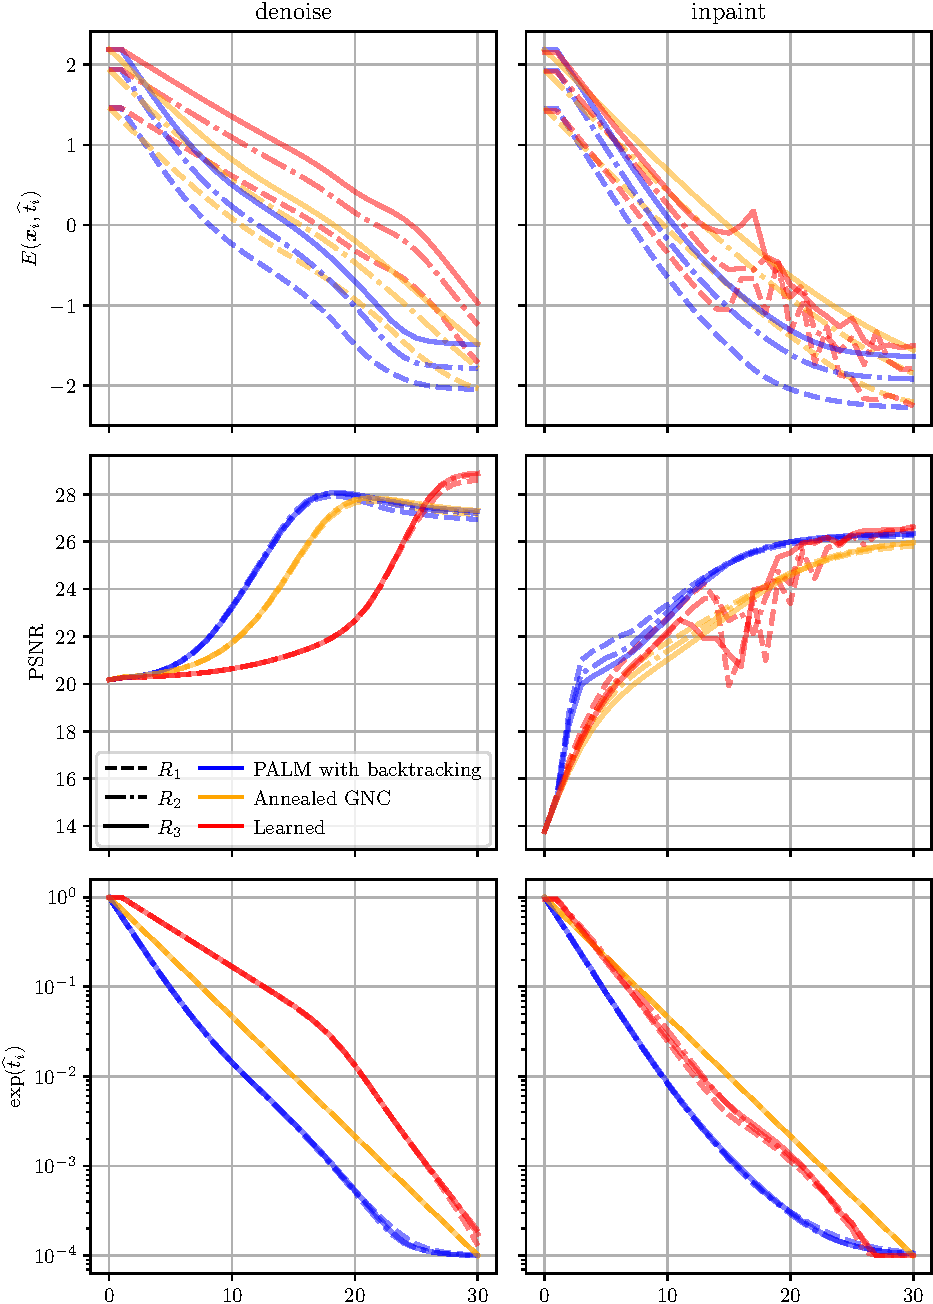
\includegraphics[width=\linewidth]{./figures/results/plots_denoise_inpaint}
% \label{fig:plotsDenoiseInpaint}
% \caption{Comparison of the different smoothing parameter schedules for image denoising (left column) and image inpainting (right column).
% The rows depict from top to bottom the energy, PSNR score, and the corresponding smoothing schedule.
% The different regularizers~$R_L$ are identified by the linestyle, whereas the smoothing parameter schedule is identified by color.
% }
% \end{figure}


\begin{figure*}[p]
\begin{tikzpicture}[every node/.append style={inner sep=1mm}, label/.style={draw=black,fill=white, inner sep=.5ex,rounded corners=1ex}]

\node[anchor=south] (r1) at (0,0) {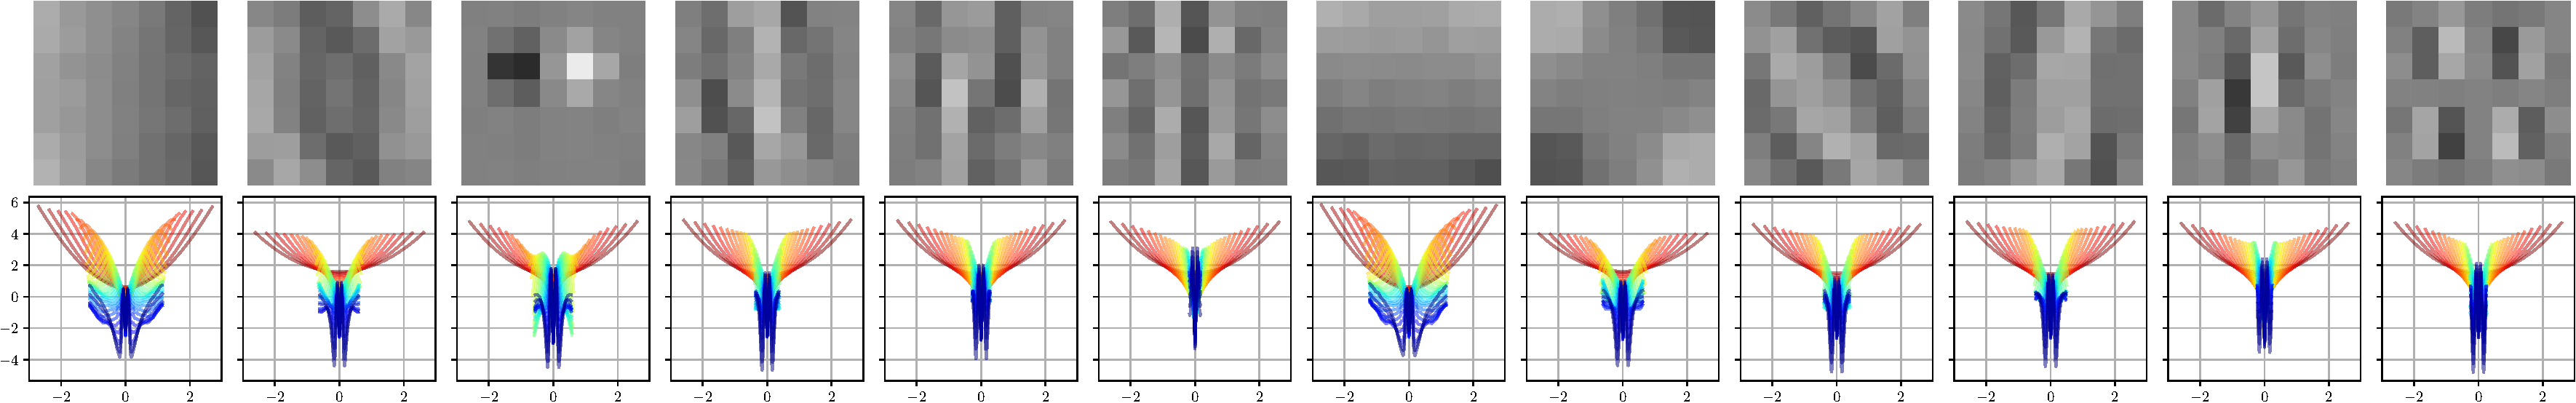
\includegraphics[width=.96\linewidth]{./figures/results/params_foe}};
\draw[black, very thick, rounded corners] (r1.north east) -- (r1.north west) -- (r1.south west) -- (r1.south east) node[midway,label,yshift=-1.25mm] {$R_1$};

\node[anchor=south] (r2) at (0,-6.25) {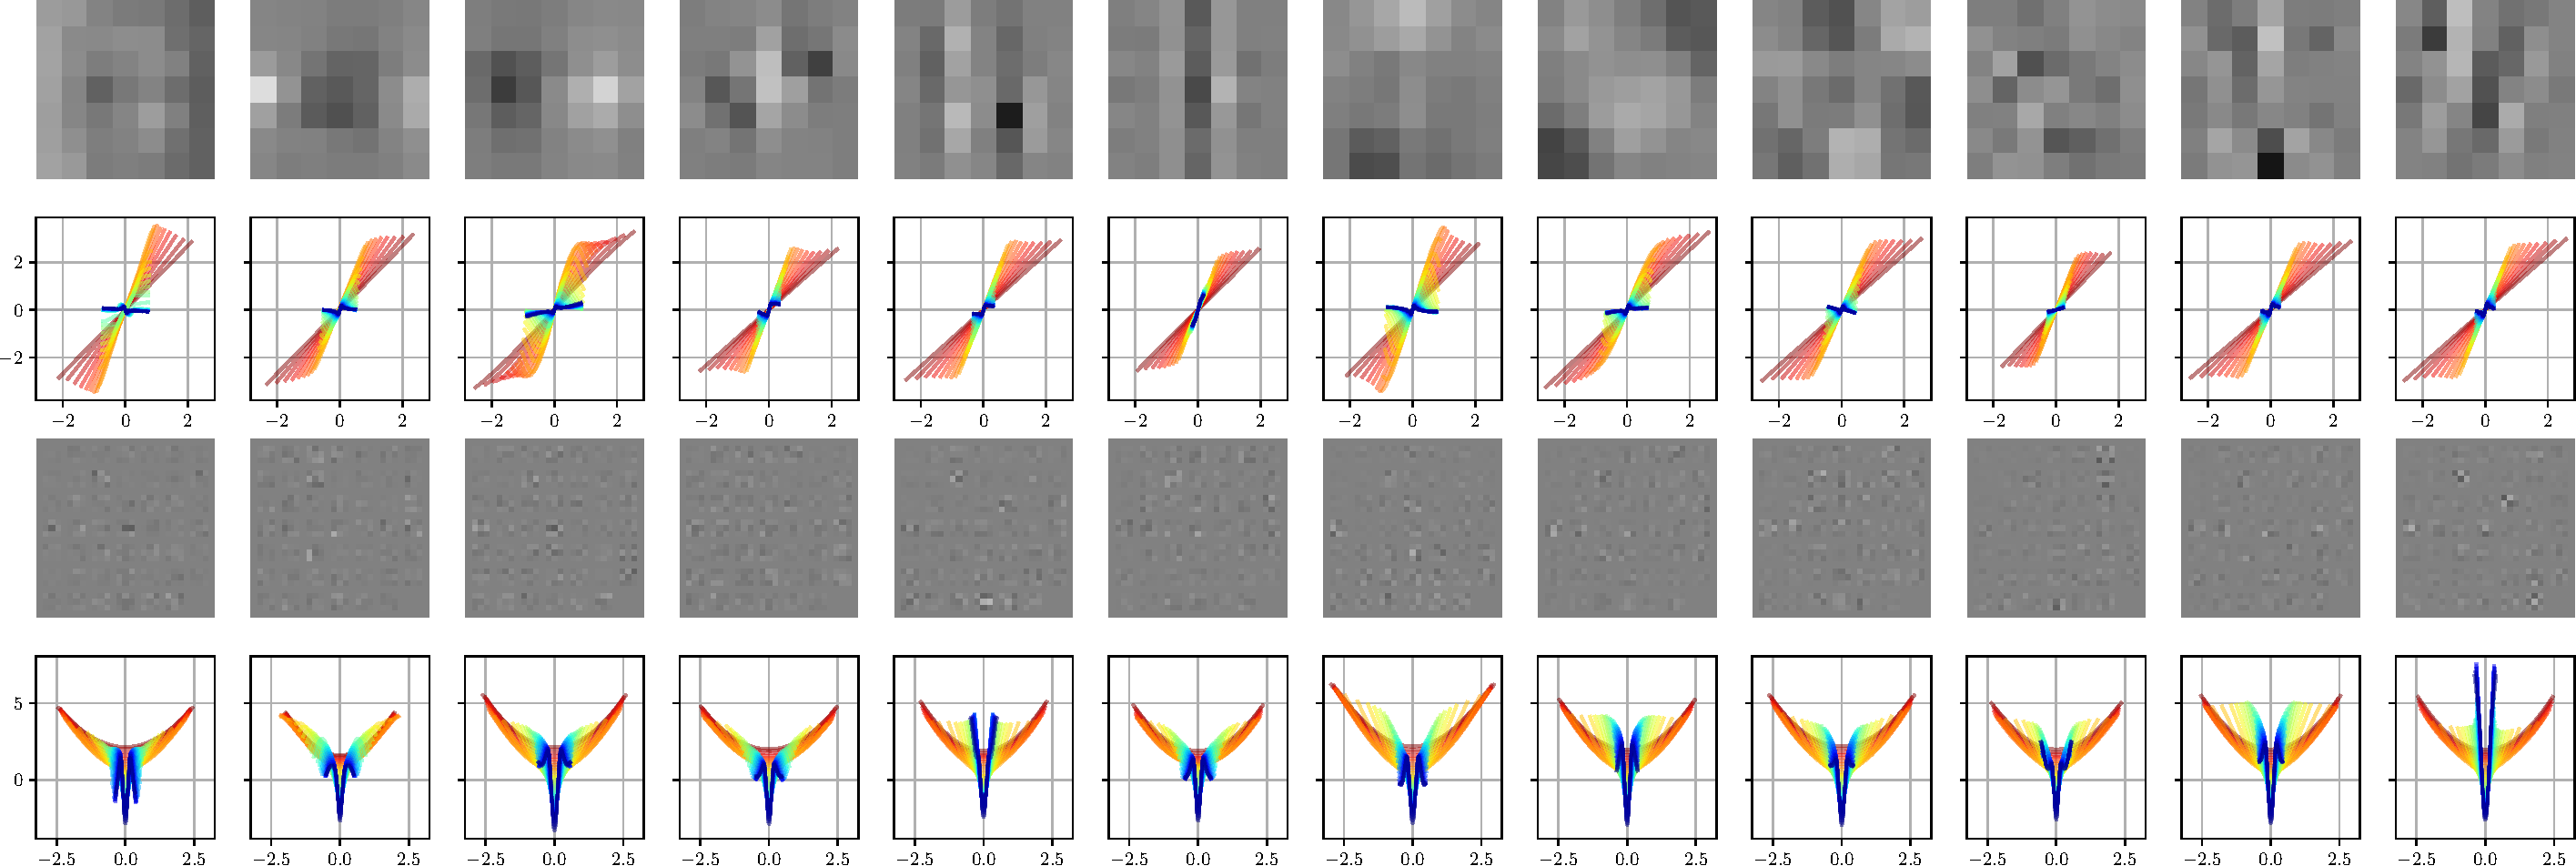
\includegraphics[width=.96\linewidth]{./figures/results/params_foedeep}};
\draw[black, very thick, rounded corners] (r2.north east) -- (r2.north west) -- (r2.south west) -- (r2.south east) node[midway,label,yshift=-1.25mm] {$R_2$};

\node[anchor=north] (r3) at (0,-6.75) {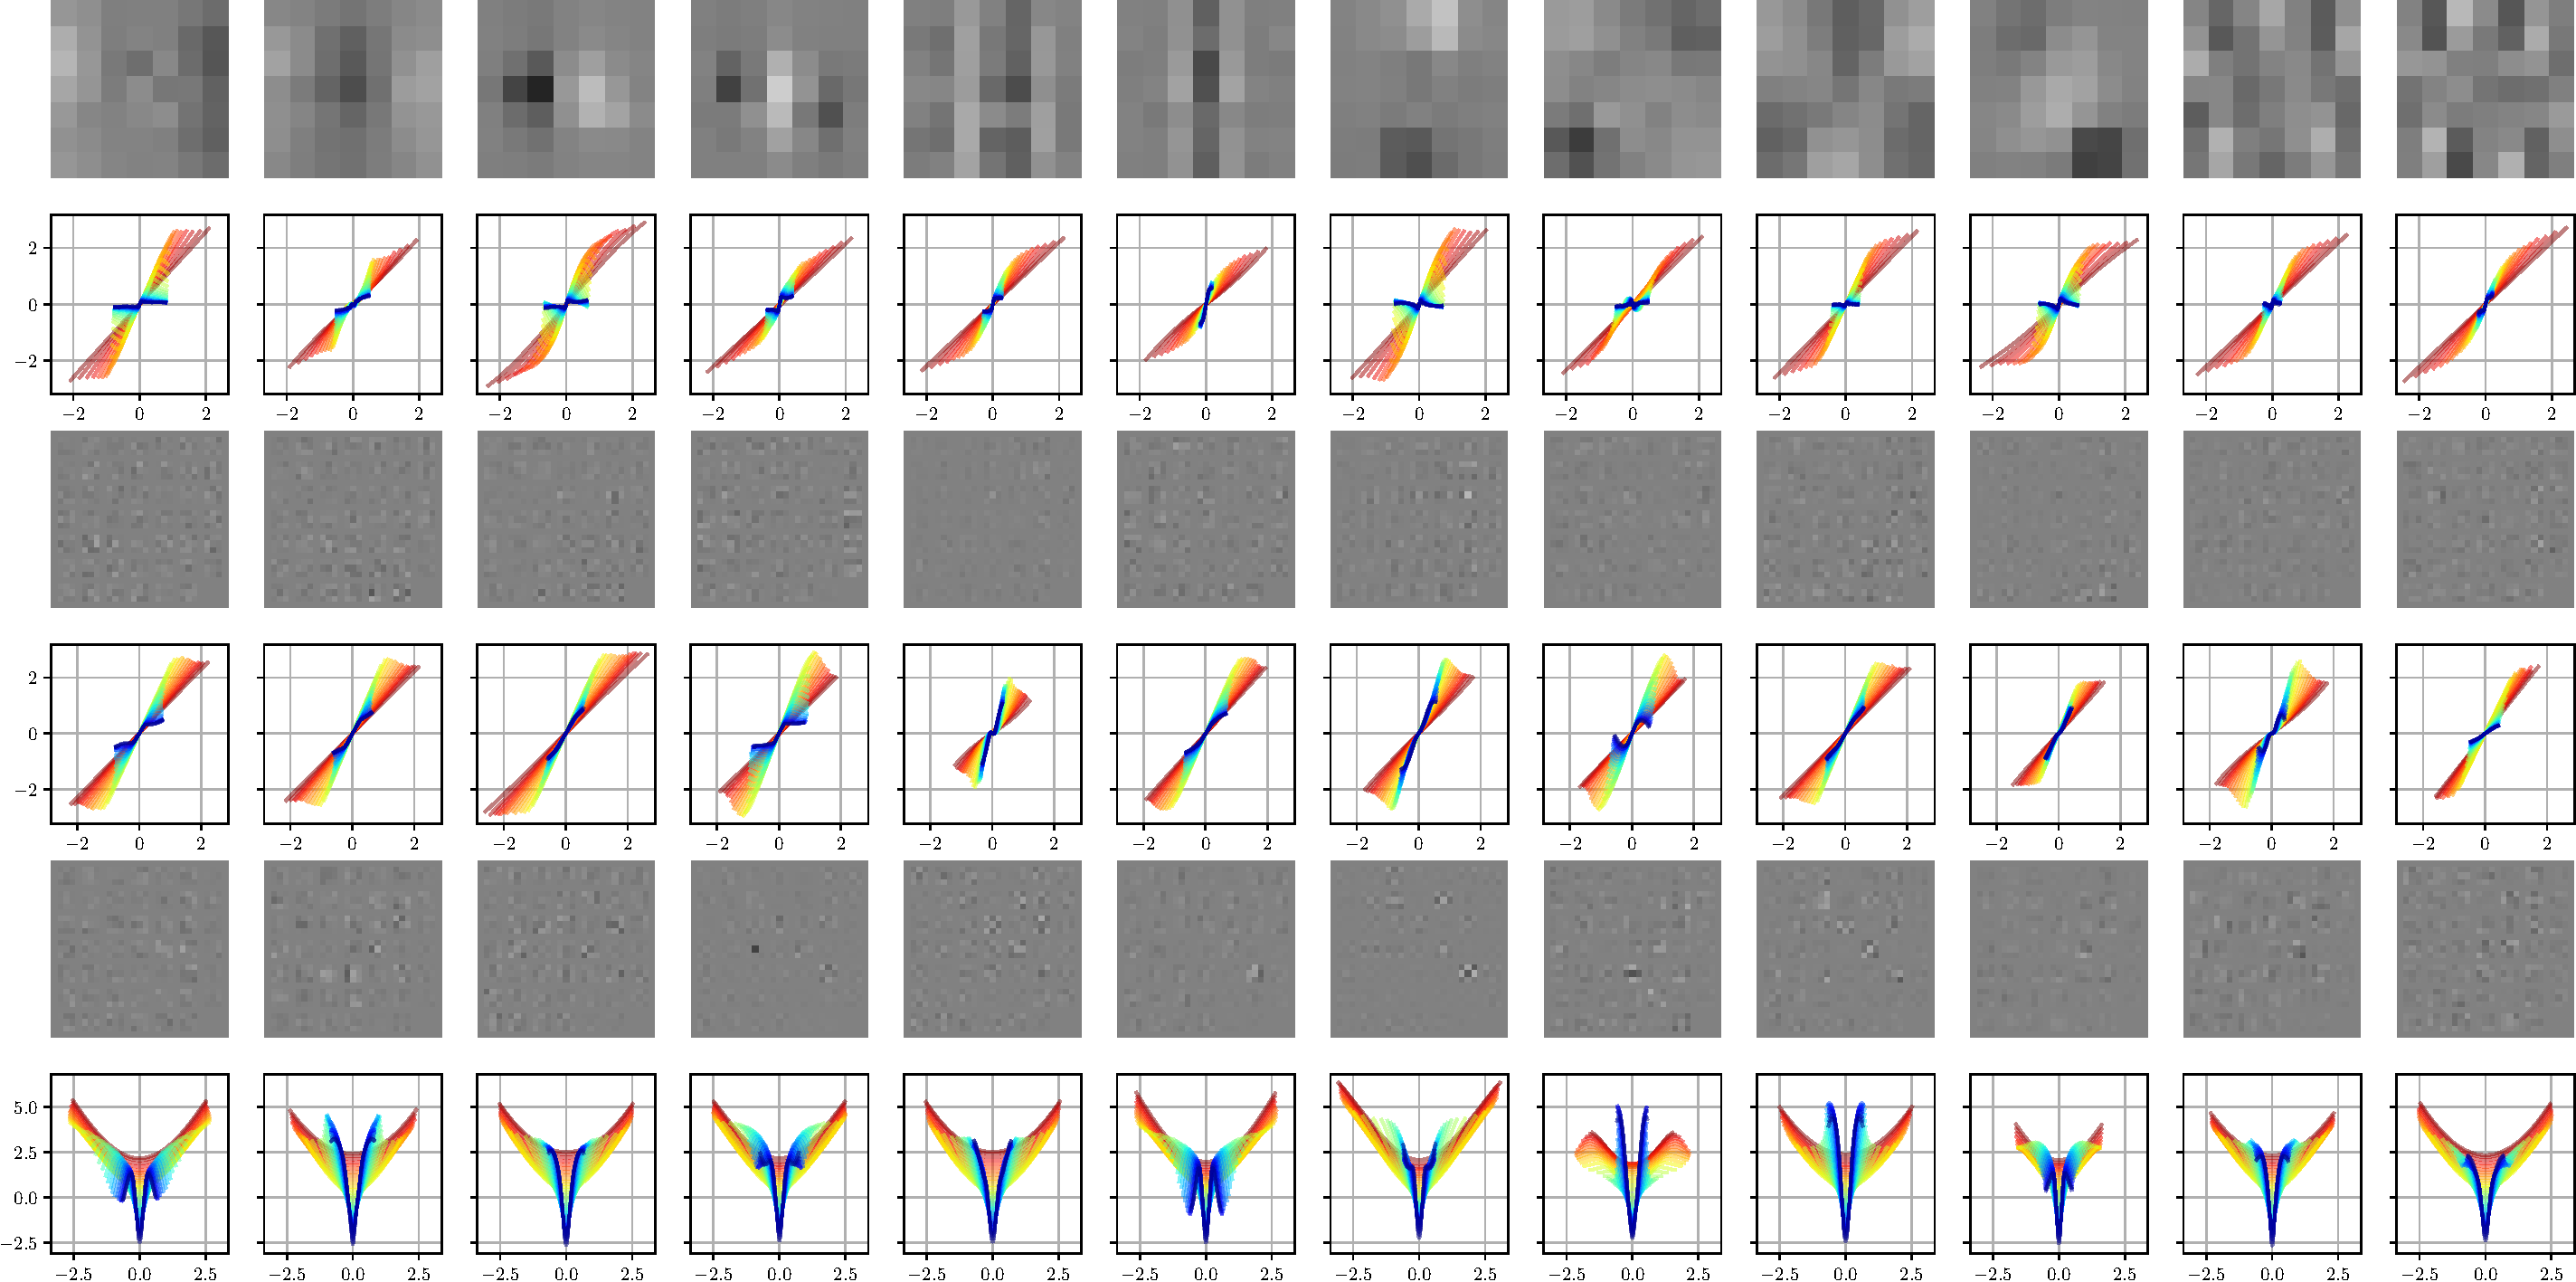
\includegraphics[width=.96\linewidth]{./figures/results/params_foedeep3}};
\draw[black, very thick, rounded corners] (r3.north east) -- (r3.north west) -- (r3.south west) -- (r3.south east) node[midway,label,yshift=-1.25mm] {$R_3$};
\end{tikzpicture}
\label{fig:paramsRegs}
\caption{
Visualization of the learned parameters of the proposed regularizers~$R_L$ for $L\in\{1,2,3\}$.\
The columns show the first $10$ features.
}
\end{figure*}

TODO:
\begin{itemize}
    \item Training on image patches
    \item 
\end{itemize}

% -----------------------------------------------------------------------------------------------------
\section{Conclusion}


\bibliography{references}
\bibliographystyle{icml2023}


%%%%%%%%%%%%%%%%%%%%%%%%%%%%%%%%%%%%%%%%%%%%%%%%%%%%%%%%%%%%%%%%%%%%%%%%%%%%%%%
%%%%%%%%%%%%%%%%%%%%%%%%%%%%%%%%%%%%%%%%%%%%%%%%%%%%%%%%%%%%%%%%%%%%%%%%%%%%%%%
% APPENDIX
%%%%%%%%%%%%%%%%%%%%%%%%%%%%%%%%%%%%%%%%%%%%%%%%%%%%%%%%%%%%%%%%%%%%%%%%%%%%%%%
%%%%%%%%%%%%%%%%%%%%%%%%%%%%%%%%%%%%%%%%%%%%%%%%%%%%%%%%%%%%%%%%%%%%%%%%%%%%%%%
\newpage
\appendix
\onecolumn

\section{Proofs of Theorem~\ref{thm:Fconvex} and Corollary~\ref{cor:empirical}} \label{apdx:proofs}

\begin{theorem}
Let~$\X\subset\R^d$ be a bounded set such that diameter~$\diameter(\X)<\infty$ and consider a GMM of the form
\[
p(\vx) = \sum_{i=1}^n w_i G(\vx_i,\Sigma_i)(\vx),
\]
where $(w_1\ \cdots \ w_n)^\top\in\Delta^n$. Assume~$\{\vx_i\}_{i=1}^n\subset\X$.
Then there exists a smoothing parameter~$\widetilde{t}\in(0,\infty)$ such that the smoothed energy
\[
F(\vx,t)\coloneqq -\log \big( (p \ast G(\vec{0}, t\id))(\vx)\big)
\]
is \emph{convex} w.r.t.~$\vx$ for all~$t\geq\widetilde{t}$.
\end{theorem}
\begin{proof}
The smoothed energy is defined as a convolution of Gaussians~\citep{Du19}, hence its explicit form reads as
\begin{align} \label{eq:fgmm}
F(\vx,t) = -\log \underbrace{\sum_{i=1}^n w_i G(\vx_i,\Sigma_i+t\id)(\vx)}_{\eqqcolon f(\vx,t)} = -\log f(\vx,t).
\end{align}
Since $F\in\C^{\infty}(\X\times \R_{++}, \R)$, the proof relies on showing positive definiteness of the Hessian~$\nabla_\vx^2 F(\vx,t)$ for any~$\vx\in\X$.
Let us first compute the gradient~$f$
\begin{align*}
\nabla_\vx f(\vx,t) &= 
-\sum_{i=1}^n \frac{w_i}{\vert 2\pi\widetilde{\Sigma}_i\vert^{\frac{1}{2}}} \exp\left(-\norm{\vx-\bm{\mu}}_{\widetilde{\Sigma}_i^{-1}}^2\right) \widetilde{\Sigma}_i^{-1} (\vx-\vx_i)\\
&= -\sum_{i=1}^n w_i G(\vx_i,\widetilde{\Sigma}_i) \underbrace{\widetilde{\Sigma}_i^{-1} (\vx-\vx_i)}_{\vr_i}
\end{align*}
using $\widetilde{\Sigma}_i = \Sigma_i+t\id$.
Similarly, the Hessian of $f$ is given by
\[
\nabla_\vx^2 f(\vx,t) = -\sum_{i=1}^n w_i G(\vx_i,\widetilde{\Sigma}_i)\left(\widetilde{\Sigma}_i^{-1} -  \vr_i\vr_i^\top\right).
\]
Then the gradient of the energy reads as
\[
\nabla_\vx F(\vx, t) = -\frac{1}{f(\vx,t)} \nabla_\vx f(\vx,t)
\]
and its Hessian is defined as
\[
\nabla_\vx^2 F(\vx, t) =
-\frac{1}{f(\vx,t)} \nabla_\vx^2 f(\vx, t) + \frac{1}{f(\vx,t)^2} \nabla_\vx f(\vx,t) \left(\nabla_\vx f(\vx,t)\right)^\top.
\]
By plugging in the Hessian of $f$, we get
\[
\nabla_\vx^2 F(\vx, t) = \underbrace{\frac{1}{f(\vx,t)}}_{\geq0}\Bigg\{\sum_{i=1}^n \underbrace{w_i G(\vx_i,\widetilde{\Sigma}_i)(\vx)}_{\geq0} \left( \widetilde{\Sigma}_i^{-1} - \vr_i\vr_i^\top  \right) + \underbrace{\frac{1}{f(\vx,t)} \nabla_\vx f(\vx,t) \left(\nabla_\vx f(\vx,t)\right)^\top}_{\succeq 0} \Bigg\}.
\]
For any~$t\in(0,\infty)$, the energy~$F$ is convex if $\nabla_\vx^2 F(\vx, t)\succeq0$ for all~$\vx\in\X$.
Since almost all parts of~$\nabla_\vx^2 F(\vx, t)$ are positive, we only need to ensure that
\[
\widetilde{\Sigma}_i^{-1} - \vr_i\vr_i^\top = \widetilde{\Sigma}_i^{-1} - \widetilde{\Sigma}_i^{-1} (\vx-\vx_i)(\vx-\vx_i)^\top \widetilde{\Sigma}_i^{-1} \succeq 0
\]
for all~$i=1,\ldots,n$.
By multiplying $\widetilde{\Sigma}_i$ from both sides, we get
\[
\widetilde{\Sigma}_i - (\vx-\vx_i)(\vx-\vx_i)^\top \succeq 0 \iff \Sigma_i + t\id \succeq (\vx-\vx_i)(\vx-\vx_i)^\top.
\]
Computing the minimal Eigenvalue on the left-hand-side and the maximal Eigenvalue on the right-hand-side, we obtain
\[
\lambda_\mathrm{min}(\Sigma_i) + t \geq \lambda_\mathrm{max}\left(\norm{\vx-\vx_i}^2 \frac{\vx-\vx_i}{\norm{\vx-\vx_i}}\frac{(\vx-\vx_i)^\top}{\norm{\vx-\vx_i}}\right) = \norm{\vx-\vx_i}^2.
\]
Since $\lambda_\mathrm{min}(\Sigma_i)\geq0$ for any $i=1,\ldots,n$, it is sufficient to show that
\[
t\geq \norm{\vx-\vx_i}^2,
\]
which is the case if 
\[
t\geq \max_{x\in\X}\max_{i=1,\ldots,n} \norm{\vx-\vx_i}^2
\]
holds true.
Note that we can estimate the right-hand-side from above by the domain's diameter~$\diameter(\X)=\sup_{x,y\in\X}\norm{x-y}$.
As a result, we conclude the proof by
\[
t\geq \diameter(\X)^2.
\]
\end{proof}

\begin{corollary}
Theorem~\ref{thm:Fconvex} also holds if an empirical discrete probability measure of a dataset~$\{\vx_i\}_{i=1}^n\subset\X$, i.e.
\[
p = \frac{1}{n}\sum_{i=1}^n\delta_{\vx_i},
\]
is considered.
Here, $\delta_{\vx}$ denotes the Dirac delta measure located at~$\vx$.
\end{corollary}

\begin{proof}
Since the convolution of the empirical probability measure~$p$ with a zero-mean Gaussian results in a GMM due to the translation property of the Dirac delta function, we get $F(\vx,t) = -\log f(\vx,t)$ for
\[
f(\vx,t)=\frac{1}{n}\sum_{i=1}^n G(\vx_i, t\id).
\]
Note that this results is identical to the definition of~$f$ in \eqref{eq:fgmm} if $\Sigma_i=\bm{0}$ for $i=1,\ldots,n$.
Consequently, the proof of this corollary follows the same line of arguments as in Theorem~\ref{thm:Fconvex}.
\end{proof}

\section{Implementation Details} \label{apdx:implementationDetails}
To extract and combine features, we use the following convolution operators.
The first convolution operator~$K_1$ facilitates~$N_1=48$ kernels of size~$7\times 7$, which are initialized by the 2D discrete cosine transform basis filers as in~\citet{ChPo16,KoKl17}.
All subsequent operators~$K_i$, $i=2,\ldots,L$ implement 2-dimensional convolutions using~$N_i=48$ kernels of size~$3\times 3$.
Those filters are initialized using ``Kaiming''-normal initialization.
Neither of the convolution operators facilitates bias terms since each subsequent non-linear parametric function may adapt to its input features.

Throughout the prior models, every non-linear function is implemented using weighted spline basis functions.
In addition, each non-linearity is a function in two variables -- an input feature~$x\in\R$ and the (logarithmic) smoothing parameter~$\widehat{t}\in[\tminh,\tmaxh]$.
For the $i^\text{th}$ layer and the $j^\text{th}$ feature channel, the output of the corresponding activation function~$\phi_{ij}$ is computed as
\[
\phi_{ij}(x,\widehat{t}) = \sum_{l=1}^{N_x}\sum_{o=1}^{N_t} w_{ij}^{lo} \varphi\left(\frac{x-\mu_x^l}{\gamma_x}\right) \varphi\left(\frac{\widehat{t}-\mu_x^o}{\gamma_t}\right),
\]
where $N_x,N_t\in\N$ define the number of basis functions and the weights~$w_{ij}^{lo}\in\R$ are learned during optimization.
For all functions, we place the means~$\mu_x^l$ on an equidistant grid on~$[-3.5,3.5]$ and set~$\gamma_x=\frac{7}{N_x-1}$.
Likewise, the means~$\mu_t^o$ are equally distributed on the interval~$[\tminh,\tmaxh]$ and $\gamma_t=\frac{\tmaxh-\tminh}{N_t-1}$.
The kernel~$\varphi\colon\R\to\R$ is given by the quartic spline, i.e.,
\[
\varphi(x)=\tfrac{1}{24}
\begin{cases}
11 + 12(\vert x\vert+\frac12) - 6(\vert x\vert+\frac12)^2 - 12(\vert x\vert+\frac12)^3 + 6(\vert x\vert+\frac12)^4 &\text{if } 0\leq\vert x\vert< \frac12\\
1 + 4(\frac32-\vert x\vert) + 6(\frac32-\vert x\vert)^2 + 4(\frac32-\vert x\vert)^3 - 4(\frac32-\vert x\vert)^4 &\text{if } \frac12\leq \vert x\vert< \frac32\\
(\frac52-\vert x\vert)^4 &\text{if } \frac32\leq \vert x\vert<\frac52\\
0 &\text{else}
\end{cases}.
\]
These activation functions are computationally much more expensive than simple ReLU-activations.
However, the spline-based activation functions are much more expressive and several implementation tricks can be used to compute these activation functions efficiently.
The non-linear functions of the intermediate layers~$\phi_i,\ i=1,\ldots,L-1$ are initialized to the identity function, while the last non-linear function~$\phi_L$ is initialized to the quadratic function.

As a source of natural image patches, we consider the BSDS500 dataset~\cite{MaFo01} and randomly extract~$96\times 96$ image patches to define the empirical distribution~$\dist{X}$.
In the implementation, we sample the smoothing parameter from a uniform distribution, i.e., $\widehat{t}\sim\mathcal{U}(\tminh,\tmaxh)$.
To minimize the training loss~\eqref{eq:losslog}, the AdaBelief~\citep{ZhTa20} optimizer is used for $100\ 000$ iterations using a mini-batch size of~$128$ along with an initial learning rate of $10^{-3}$.
The learning rate is annealed to~$5\cdot 10^{-5}$ using a cosine scheme.
We utilize the AdaBelief optimizer since it performs preconditioning based on local curvature information.
Thus, it is well suited to learn parameters that lie in different intervals.

%%%%%%%%%%%%%%%%%%%%%%%%%%%%%%%%%%%%%%%%%%%%%%%%%%%%%%%%%%%%%%%%%%%%%%%%%%%%%%%
%%%%%%%%%%%%%%%%%%%%%%%%%%%%%%%%%%%%%%%%%%%%%%%%%%%%%%%%%%%%%%%%%%%%%%%%%%%%%%%


\end{document}


% This document was modified from the file originally made available by
% Pat Langley and Andrea Danyluk for ICML-2K. This version was created
% by Iain Murray in 2018, and modified by Alexandre Bouchard in
% 2019 and 2021 and by Csaba Szepesvari, Gang Niu and Sivan Sabato in 2022. 
% Previous contributors include Dan Roy, Lise Getoor and Tobias
% Scheffer, which was slightly modified from the 2010 version by
% Thorsten Joachims & Johannes Fuernkranz, slightly modified from the
% 2009 version by Kiri Wagstaff and Sam Roweis's 2008 version, which is
% slightly modified from Prasad Tadepalli's 2007 version which is a
% lightly changed version of the previous year's version by Andrew
% Moore, which was in turn edited from those of Kristian Kersting and
% Codrina Lauth. Alex Smola contributed to the algorithmic style files.
